% Chapter 6

\begin{savequote}[45mm]
Coconut oil for your skin \ldots
\qauthor{Polynesian proverb}
\end{savequote}

\chapter{Investigating biodiesel feedstock by SFC×GC} % Main chapter title

\label{Chapter6} % For referencing this chapter elsewhere, use \ref{Chapter6}


\section{Introduction}

Biodiesel is composed of a mixture of methyl esters of fatty acids obtained from
plant oils \autocite{SANS1935}. To comply with the relevant standard
\autocite{SANS1935}, (See chapter 3), it must consists of a mass fraction of
\SI{96.5}{\percent} or more of methyl esters, and it must have fewer than a
certain amount of specific unsaturated fatty acids methyl esters.

The methods for determining fatty acid methyl esters are chromatographic. Each
limit has its own method, and it therefore becomes expensive to determine each
of them.
 
Both these methods generate complex chromatograms that need highly skilled and
experienced chromatographers to interpret. Each peak in the chromatogram has a
retention time and area, which needs to be interpreted. There is no doubt that
the use of artificial intelligence and other technological innovation for
interpreting chromatograms will grow \todo{Cite AI chromatogram
interpretation.}, but the paradox of automation (automation helps you least when
you need it most\todo{autocite Automation paradox Strauch2018 Bainbridge1983})
predicts that as biodiesel production grows, with the implied increase in
complexity as feedstocks differentiate, the analytical chemist will need better
chemistry, in addition to better automatic data analysis.

Comprehensively coupled chromatography offers a way to better exploit chemistry
for improved separations. It does this in three ways: the first is increasing
the peak capacity of the system, the second is by improved sensitivity, and the
third is by generating patterns in the data.


\section{SFC of FAMEs}

The power of comprehensive chromatography is unlocked by orthogonality.
Orthogonality is the difference is separation mechanism in the two dimensions
\todo{autocite{LGGC nomenclature}}. When fatty acid methyl esters are separated
by a system using pure carbon dioxide as a mobile phase and unmodified silica as
a stationary phase, then the separation is according to the number of double
bonds, independent of chain length \autocite{Robertson1991, Smith1994,
Smith2001}. This is in strong contrast to the separation of FAME by GC, where
the major separation is according to volatilty, which can be adjusted, but not
overridden, by changing the polarity (or other chemical aspect) of the mobile
phase.

\begin{figure}
\centering
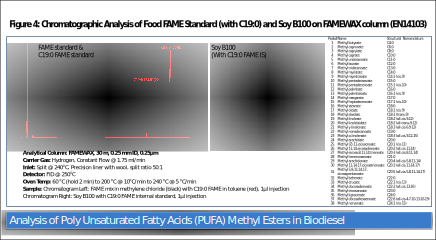
\includegraphics[width=\textwidth]{Figures/FAME-GC.pdf}
\decoRule

\caption[Separation of FAME by GC]{This figure shows that when separating FAME
by GC, using specialized column, separation is primarily by fatty acid chain
length, and secondarily by number of double bonds.The peaks elute }

\label{fig:co2fill}
\end{figure}

Silver ions are often used in stationary phases to separate unsaturated
compounds, and this includes stationary phases for SFC \autocite{Sandra2002,
Potgieter2013}. The retention mechanism is quite complex
\autocite{Nikolova-Damyanova2019}, but it offers a powerful technique for the
elucidation of lipid structures, as reviewed as early as 1966
\autocite{Morris1966}. Nevertheless, in this chapter the use of stationary
phases modified with silver ions was neither necessary nor attempted.

The low viscosity of the carbon dioxide mobile phase allows for the use of very long
columns \autocite{Smith2001}.

As discussed in Section \ref{sec:Rancimat}, fatty acids are not stable at high
temperatures. This means that they might degrade during chromatographic
separation at high temperature, especially if the run times are long. Because
SFC operates at low temperatures, the labile compounds are less likely to degrade. 

\section{CG of FAME}

As discussed in Section \label{sec:ChromDet}, FAME can be separated by gas
chromatography using a relatively non-polar columns using high-temperature
programs.
 
Short columns and fast temperature programs have a beneficial side effect:
reduced \keyword{column bleed}. Any resin- or polymer-based stationary phase
degrades over time, and this degradation is faster at higher temperatures
\autocite[p. 66]{Mcnair2019}. It is observed as a rise in baseline during the
high temperature part of a temperature program. Various stationary phase
technologies can be employed to reduce column bleed, but it should be obvious
that a \SI{1}{\metre} column will have \num{1/30}th \todo{fix ordinal} of the
column bleed of a \SI{30}{\metre} column. (It should be noted that the column
lifetime will not be longer, just that the increase in baseline signal from
column bleed will be lower.)



